\documentclass[10pt,a4paper]{article}
\usepackage[T1]{fontenc}
\usepackage[utf8]{inputenc}
\usepackage[french]{babel}
\usepackage{lmodern}
\usepackage[top=16mm,bottom=16mm,left=15mm,right=15mm,headheight=13pt,headsep=5mm,footskip=8mm]{geometry}
\usepackage{amsmath,amssymb,array,booktabs,tabularx,graphicx,xcolor}
\usepackage{tikz}
\usetikzlibrary{arrows.meta,positioning,calc}
\usepackage{fancyhdr}
\usepackage[hidelinks]{hyperref}
\definecolor{navy}{HTML}{17364E}
\definecolor{pale}{HTML}{EDF2F6}
\definecolor{muted}{HTML}{52616D}
\definecolor{rulegray}{HTML}{CBD3DA}
\hypersetup{pdftitle={ResilientInspect AI - Rapport de mi-parcours},pdfauthor={Nouha Ben Khelil et Nouha Briki},pdfsubject={Deep Learning Avance - TEK-UP University}}
\pagestyle{fancy}
\fancyhf{}
\fancyhead[L]{\small\color{muted}ResilientInspect AI}
\fancyhead[R]{\small\color{muted}Deep Learning Avancé -- Mi-parcours}
\fancyfoot[L]{\small\color{muted}TEK-UP University \quad 2026--2027}
\fancyfoot[R]{\small\thepage/5}
\renewcommand{\headrulewidth}{0.3pt}
\setlength{\parindent}{0pt}
\setlength{\parskip}{3pt}
\setlength{\tabcolsep}{4pt}
\renewcommand{\arraystretch}{1.13}
\setlength{\emergencystretch}{1.5em}
\raggedbottom
\makeatletter
\renewcommand\section{\@startsection{section}{1}{0pt}{7pt}{4pt}{\large\bfseries\color{navy}}}
\renewcommand\subsection{\@startsection{subsection}{2}{0pt}{6pt}{3pt}{\normalsize\bfseries\color{navy}}}
\makeatother
\newcommand{\todo}{\textbf{\textcolor{navy}{[À COMPLÉTER]}}}
\newcommand{\source}[1]{\par{\fontsize{8.5}{10}\selectfont\color{muted}\raggedright #1\par}}
\newcommand{\status}[1]{\par\noindent\fcolorbox{rulegray}{pale}{\parbox{\dimexpr\linewidth-2\fboxsep-2\fboxrule\relax}{\small #1}}\par}
\newcommand{\proofcaption}[1]{\par{\small\color{muted}#1\par}}
\newcolumntype{Y}{>{\raggedright\arraybackslash}X}
\newcolumntype{C}{>{\centering\arraybackslash}X}
\begin{document}

{\small\color{muted}\textbf{RAPPORT ACADÉMIQUE DE MI-PARCOURS}\hfill Suivi technique : 20\,\% de la note du projet\par}
{\fontsize{21}{24}\selectfont\bfseries\color{navy}ResilientInspect AI\par}
{\large Détection et localisation d'anomalies industrielles par Deep Learning\par}
{\small Enseignant : Haythem Ghazouani \hfill État audité le 11 novembre 2026\par}

\section{Fiche d'identité et état global du projet}
\par\begin{tabularx}{\linewidth}{@{}p{32mm}Y@{}}
\textbf{Track métier} & Vision industrielle -- CNN et Transfer Learning ; code officiel \textbf{TrackX} : \todo.\\
\textbf{Groupe} & Numéro / identifiant officiel : \todo.\\
\textbf{Dépôt Git} & \url{https://github.com/nouhabenkhelil/resilientinspect-ai}\\
\textbf{Suivi MLflow} & Interface locale \url{http://127.0.0.1:5000/} ; bases et artefacts rapatriés de Kaggle.\\
\end{tabularx}
\par\begin{tabularx}{\linewidth}{@{}p{34mm}p{65mm}Y@{}}
\toprule
\textbf{Étudiante} & \textbf{Courriel} & \textbf{Rôle individuel confirmé}\\
\midrule
Nouha Ben Khelil & \texttt{nouhebenkhelil@gmail.com} & \todo\\
Nouha Briki & \texttt{brikinouha2@gmail.com} & \todo\\
\bottomrule
\end{tabularx}
\status{\textbf{Avancement global estimé : 50\,\%.} Notre socle expérimental est opérationnel : données préparées, six entraînements AE complets et évaluations B0/A1 disponibles. Le transfert complet et les services applicatifs restent à livrer. Cette estimation de planification est justifiée en section 2 ; elle ne mesure ni la qualité des modèles ni la note attendue.}

\textbf{Sujet et objectifs.} Nous cherchons à détecter une image industrielle anormale et à localiser les zones suspectes, afin d'appuyer un contrôle visuel reproductible. Nous comparons un autoencodeur de référence B0 à une version A1 plus expressive, puis préparons une expérience de transfert T0/T1/T2. Nous ne prétendons pas remplacer une validation industrielle : notre étude porte sur trois catégories MVTec AD et sur leurs conditions d'acquisition.

\begin{center}
\begin{tikzpicture}[x=1mm,y=1mm,>=Latex,
 done/.style={draw=navy,fill=pale,rounded corners=1mm,text width=34mm,minimum height=11mm,align=center,font=\small},
 future/.style={done,draw=muted,dashed,fill=white,text=muted},
 link/.style={->,draw=navy,thick}]
\node[done] (data) at (19,0) {MVTec AD\\3 catégories};
\node[done] (audit) at (63,0) {Audit d'intégrité\\et EDA};
\node[done] (prep) at (107,0) {Préparation\\Manifestes SHA256};
\node[done] (loader) at (151,0) {PyTorch\\DataLoader};
\node[done] (models) at (151,-20) {Modèles\\B0 / A1};
\node[done] (gpu) at (85,-20) {Entraînement\\Kaggle Tesla T4};
\node[done] (track) at (19,-20) {MLflow\\et checkpoints};
\node[done] (eval) at (19,-40) {Évaluation\\et heatmaps};
\node[done] (compare) at (85,-40) {Comparaison\\B0 / A1};
\node[future] (deploy) at (151,-40) {Déploiement futur\\API et interface};
\foreach \a/\b in {data/audit,audit/prep,prep/loader,loader/models,models/gpu,gpu/track,track/eval,eval/compare}{\draw[link] (\a)--(\b);}
\draw[link,dashed] (compare)--(deploy);
\end{tikzpicture}
\end{center}
\proofcaption{Figure 1 -- Pipeline réellement développé. Les blocs bleutés sont réalisés ; le bloc en pointillés reste prévu. La branche auxiliaire T0/T1/T2 est implémentée et vérifiée en smoke CPU, sans entraînement complet local confirmé.}

\section{Travail déjà réalisé}
\subsection{Données et versioning DVC}
Nous avons retenu \textit{bottle} (objets rigides), \textit{hazelnut} (objets naturels) et \textit{leather} (textures et surfaces) pour explorer des défauts différents, sans couvrir tout MVTec AD. Nous avons contrôlé les fichiers, les masques et leurs appariements avant de figer les partitions.
\par\begin{tabularx}{\linewidth}{@{}Yrrrrr@{}}
\toprule
\textbf{Catégorie} & \textbf{Images} & \textbf{Train normal} & \textbf{Val normale} & \textbf{Test} & \textbf{Masques}\\
\midrule
bottle & 292 & 167 & 42 & 83 & 63\\
hazelnut & 501 & 312 & 79 & 110 & 70\\
leather & 369 & 196 & 49 & 124 & 92\\
\textbf{Total} & \textbf{1 162} & \textbf{675} & \textbf{170} & \textbf{317} & \textbf{225}\\
\bottomrule
\end{tabularx}
\source{Sources : \texttt{reports/eda/audit\_summary.csv}, \texttt{data/manifests/manifest.csv} et \texttt{reports/experiments/data\_preparation.json}. Test : 92 images normales et 225 anormales.}
Nous réservons environ 20\,\% du \texttt{train/good} officiel à la validation, par catégorie, avec seed 42 et arrondi supérieur. Les images deviennent RGB dans $[0,1]$, en letterbox $256\times256$ : interpolation bilinéaire pour le RGB, nearest-neighbor pour les masques. Les manifestes CSV, les images et les checkpoints sont contrôlés par SHA256. Le test officiel n'entre pas dans l'entraînement des AE. \textbf{DVC n'est pas configuré} ; les empreintes assurent actuellement la traçabilité, sans constituer un versioning DVC opérationnel.

\newpage
\subsection{Modélisation et entraînement Deep Learning}
\textbf{B0 : une référence par reconstruction.} Nous entraînons un encodeur--décodeur à reconstruire les seules images normales. L'encodeur compresse l'information, puis le décodeur restitue une image RGB. Une erreur élevée à la reconstruction peut signaler une anomalie, mais ce mécanisme n'assure pas que tout défaut sera mal reconstruit. B0 compte \textbf{195 107 paramètres} et minimise la perte L1.

\textbf{A1 : une capacité accrue à examiner.} Nous ajoutons des blocs résiduels, qui facilitent la propagation de l'information et des gradients. Des skips limités aux résolutions $32^2$ et $64^2$, avec contribution bornée à $\pm0{,}1$, aident à restituer la structure sans chemin RGB direct. A1 compte \textbf{2 754 371 paramètres}. Sa perte est $0{,}8\,\mathrm{L1}+0{,}2\,\mathrm{DSSIM}$, où $\mathrm{DSSIM}=(1-\mathrm{SSIM})/2$ mesure une dissimilarité structurelle locale. SSIM compare localement luminance, contraste et structure, tandis que L1 pénalise les écarts absolus entre pixels. Nous appliquons de faibles variations de luminosité et de contraste uniquement sur train. Des skips contrôlés ne suppriment pas le risque de recopier un défaut.

\begin{center}
\begin{tikzpicture}[x=1mm,y=1mm,>=Latex,
 block/.style={draw=navy,fill=pale,rounded corners=1mm,align=center,font=\small,minimum height=11mm},
 arrow/.style={->,draw=navy}]
\node[font=\bfseries,text=navy] at (4,0) {B0};
\node[block,text width=22mm] (b0in) at (26,0) {RGB\\$3\times256^2$};
\node[block,text width=38mm] (b0enc) at (66,0) {Encodeur Conv--BN--ReLU\\16 / 32 / 64 / 128};
\node[block,text width=27mm] (b0lat) at (108,0) {Latent\\$128\times16^2$};
\node[block,text width=40mm] (b0dec) at (152,0) {Upsampling + Conv\\RGB Sigmoid};
\draw[arrow] (b0in)--(b0enc);\draw[arrow] (b0enc)--(b0lat);\draw[arrow] (b0lat)--(b0dec);
\node[font=\bfseries,text=navy] at (4,-29) {A1};
\node[block,text width=22mm] (a1in) at (26,-29) {RGB\\$3\times256^2$};
\node[block,text width=38mm] (a1enc) at (66,-29) {Conv + blocs résiduels\\32 / 64 / 128 / 256};
\node[block,text width=27mm] (a1lat) at (108,-29) {Latent\\$256\times16^2$};
\node[block,text width=40mm] (a1dec) at (152,-29) {Décodeur résiduel\\RGB Sigmoid};
\draw[arrow] (a1in)--(a1enc);\draw[arrow] (a1enc)--(a1lat);\draw[arrow] (a1lat)--(a1dec);
\draw[arrow,dashed] (a1enc.north)--++(0,7)--node[above,font=\small,fill=white]{Skips $32^2/64^2$ contrôlés}(152,-16)--(a1dec.north);
\end{tikzpicture}
\end{center}
\proofcaption{Figure 2 -- Schéma comparatif des deux AE. Les détails d'architecture sont fixés dans \texttt{ae\_baseline.yaml} et \texttt{ae\_improved.yaml}. Le coût en paramètres n'est pas une preuve de supériorité.}

\textbf{Comparabilité.} Nous conservons les mêmes sources, splits et seed 42 : Adam, LR $0{,}001$, batch 16, maximum 20 époques, patience 5, FP32 sans AMP. Chaque catégorie possède son propre modèle. Le meilleur checkpoint minimise la perte val correspondante. \textbf{Nous ne comparons pas directement les pertes B0 et A1}, car leurs objectifs diffèrent.

\textbf{Exécution Kaggle confirmée.} L'absence de GPU NVIDIA CUDA local nous a conduites à entraîner sur Kaggle. Les six environnements archivés indiquent une \textbf{Tesla T4}, Python 3.13.16 et PyTorch 2.11.0+cu130. Nous avons préservé le runtime CUDA préinstallé, exécuté les configurations et récupéré historiques, poids et provenance. Les six checkpoints complets du 8 novembre sont cohérents avec les manifestes et les runs MLflow ; les smoke et copies d'artefacts sont exclus du décompte.

\par\begin{tabularx}{\linewidth}{@{}p{20mm}CCC@{}}
\toprule
\textbf{AE} & \textbf{bottle} & \textbf{hazelnut} & \textbf{leather}\\
\midrule
B0 & 19 / 20 & 18 / 20 & 14 / 19\\
A1 & 15 / 20 & 17 / 20 & 18 / 20\\
\bottomrule
\end{tabularx}
\source{Époques : meilleure / réalisées. Sources : \texttt{artifacts/\{b0,a1\}\_runs/<catégorie>/full\_<runid>/}, fichiers \texttt{summary.json}, \texttt{history.csv}, \texttt{environment.json} et \texttt{best.pt}. Arrêt anticipé effectif à 19 époques pour B0 leather.}

\textbf{Évaluation figée.} Pour une image $x$ et sa reconstruction $\hat x$, nous calculons la carte $e_{ij}=\frac{1}{3}\sum_c|x_{cij}-\hat x_{cij}|$, sans lissage, à $256^2$. Le score image est la moyenne du top 1\,\% des pixels valides. Les seuils sont recalculés par modèle sur les seules validations normales : quantile 95\,\% image et 99,5\,\% pixel, méthode \texttt{higher}, décision strictement $>$. Le padding est exclu. Nous utilisons le test uniquement pour l'évaluation finale, jamais pour choisir ces seuils.

\textbf{Transfert : code validé, expérience complète à réaliser.} Nous avons implémenté EfficientNet-B0 : T0 depuis zéro, T1 ImageNet gelé et T2 avec dégel des stages 6--8. La tête binaire et la normalisation ImageNet sont communes. Les anomalies synthétiques localisées sont fixées à partir de train/good et, séparément, de val/good, sans source partagée entre splits. Les trois variantes ont seulement des smoke CPU locaux confirmés. Grad-CAM explique leur logit via \texttt{features.8.0} ; nous ne le présentons pas comme une segmentation pixel.

\status{\textbf{Développement vérifié, sans nouvelle exécution pour ce rapport.} La preuve du 9 novembre consigne 462 tests réussis et deux tests CUDA ignorés sur la machine CPU, dont 119 nouveaux cas transfert. Trois smoke T0/T1/T2 sur images artificielles ont chacun effectué deux pas Adam. Leurs métriques ne mesurent pas une performance industrielle.}
\source{Preuve : \texttt{reports/experiments/transfer\_implementation\_verification.json} et tests du dépôt. Pas de capture d'écran des tests disponible : nous nous appuyons sur cette preuve JSON, sans fabriquer d'image.}

\newpage
{\large\bfseries\color{navy}Résultats expérimentaux vérifiés\par}
Les résultats de \textbf{B0 et A1 sont disponibles sur les trois catégories}. Nous utilisons les CSV et JSON d'évaluation présents, qui partagent le même protocole, le même manifeste, les mêmes labels et les mêmes pixels test. Les 317 images test sont réparties en 83 bottle, 110 hazelnut et 124 leather. La classe positive est l'anomalie. AUROC et AP (Average Precision) décrivent le classement continu ; F1, Dice et IoU décrivent les décisions aux seuils val.

\textbf{Tableau 1 -- Classification image.}\quad Valeurs recopiées sans arrondi.
{\fontsize{9.2}{11}\selectfont
\par\begin{tabularx}{\linewidth}{@{}p{21mm}p{9mm}CCC@{}}
\toprule
\textbf{Catégorie} & \textbf{AE} & \textbf{AUROC image} & \textbf{AP image} & \textbf{F1 image}\\
\midrule
bottle & B0 & 0.711111111111111 & 0.9083742437626401 & 0.6666666666666666 \\
bottle & A1 & 0.8071428571428572 & 0.9430503235681029 & 0.7524752475247525 \\
hazelnut & B0 & 0.9317857142857143 & 0.9622706873152496 & 0.7387387387387387 \\
hazelnut & A1 & 0.9375 & 0.9647752847372622 & 0.2716049382716049 \\
leather & B0 & 0.7479619565217392 & 0.9142280025396583 & 0.8465116279069768 \\
leather & A1 & 0.6243206521739131 & 0.8722523808559657 & 0.7195767195767195 \\
\midrule
Macro & B0 & 0.7969529273061883 & 0.9282909778725159 & 0.7506390111041273 \\
Macro & A1 & 0.78965450310559 & 0.926692663053777 & 0.5812189684576924 \\
\bottomrule
\end{tabularx}\par}
\vspace{3pt}
\textbf{Tableau 2 -- Classement pixel et recouvrement des masques.}
{\fontsize{9.2}{11}\selectfont\setlength{\tabcolsep}{2.5pt}
\par\begin{tabularx}{\linewidth}{@{}p{18mm}p{6mm}CCCC@{}}
\toprule
\textbf{Catégorie} & \textbf{AE} & \textbf{AUROC pixel} & \textbf{AP pixel} & \textbf{Dice micro} & \textbf{IoU micro}\\
\midrule
bottle & B0 & 0.7524252739997918 & 0.14552464697702774 & 0.07864995275731841 & 0.04093473381916456 \\
bottle & A1 & 0.7700283377669875 & 0.18706906073361584 & 0.09403809497307751 & 0.04933891633670883 \\
hazelnut & B0 & 0.9341740761964867 & 0.5054197137876925 & 0.504390485859768 & 0.3372474439959166 \\
hazelnut & A1 & 0.9136788453977694 & 0.49894390034626174 & 0.264750512266711 & 0.1525720158042217 \\
leather & B0 & 0.8329733750269519 & 0.2013103350338791 & 0.13959787852455577 & 0.07503640041747736 \\
leather & A1 & 0.7474264505125233 & 0.12004666234065733 & 0.07410377524762946 & 0.03847755361645077 \\
\midrule
Macro & B0 & 0.8398575750744101 & 0.28408489859953306 & 0.24087943904721407 & 0.15107285941085283 \\
Macro & A1 & 0.8103778778924268 & 0.26868654114017826 & 0.14429746082913933 & 0.08012949525246044 \\
\bottomrule
\end{tabularx}\par}
\source{Sources exactes : \texttt{reports/evaluation/}, sous-dossiers \texttt{b0} et \texttt{a1}, protocole \texttt{f515662ab4ef}.\newline Fichiers : \texttt{category\_metrics.csv}, \texttt{macro\_metrics.json} et les six \texttt{<catégorie>/metrics.json} ; copie dans \texttt{audit/metrics\_exact.csv}. Macro : moyenne non pondérée des trois catégories ; Dice/IoU micro : agrégation TP/FP/FN des pixels valides de chaque catégorie.}

\textbf{Interprétation.} A1 progresse sur les sept métriques pour bottle. Sur hazelnut, son classement image progresse légèrement, mais le F1 et le recouvrement baissent : au seuil val fixé, les vrais positifs image passent de 41 à 11, et les faux négatifs de 29 à 59, sans faux positif pour les deux AE. Sur leather, les sept métriques diminuent. Le F1 élevé de B0 leather doit lui-même être nuancé : les 32 normales test sont toutes prédites anormales. Nous distinguons donc classement et décision seuillée. Les moyennes macro ne démontrent \textbf{aucune supériorité globale d'A1}. Une seule réalisation par catégorie, sans intervalle de confiance, ne permet ni conclusion de significativité ni attribution causale aux skips ou à SSIM sans ablation.

\subsection{Tracking MLflow}
Nous avons enregistré les configurations, train\_loss/val\_loss par époque, meilleurs checkpoints, courbes et identifiants. Les bases locales confirment \textbf{six runs AE complets FINISHED}, trois B0 et trois A1, dans \texttt{resilientinspect-ae}. Nous distinguons les \textbf{six smoke} supplémentaires : un B0, deux A1 et trois transfert ; ils ne constituent pas des entraînements complets. Les fichiers et les séries de pertes concordent avec les bases SQLite. Les URI d'origine Kaggle restent archivées ; leurs copies locales ont été retrouvées et contrôlées.

La capture de l'annexe A montre trois B0 complets et un smoke. Son nom, \texttt{6\_runs\_mlflow.png}, ne prouve pas six entraînements. La confirmation des trois A1 vient des checkpoints et de \texttt{artifacts/a1\_runs/mlflow.db}.

\subsection{FastAPI et frontend}
Nous avons privilégié les expériences Deep Learning. \textbf{FastAPI et l'interface ne sont pas implémentés} : backend, frontend et workflows CI contiennent seulement des emplacements réservés. Nous n'annonçons donc ni \texttt{/health}, ni \texttt{/predict}, ni Swagger comme fonctionnels. DVC, export ONNX, Docker et CI/CD restent à intégrer. Le tracking MLflow opérationnel ne constitue pas une chaîne de déploiement complète.

\newpage
{\large\bfseries\color{navy}Avancement par composant\par}
{\small
\par\begin{tabularx}{\linewidth}{@{}p{29mm}rYY@{}}
\toprule
\textbf{Composant} & \textbf{Estimé} & \textbf{Éléments réalisés} & \textbf{Prochaine preuve attendue}\\
\midrule
Données et DVC & 70\,\% & Audit, splits, manifestes SHA256 & DVC initialisé et reproductible\\
Modélisation DL & 80\,\% & B0/A1 entraînés et évalués ; transfert codé & Neuf runs transfert full puis test réel\\
MLflow & 80\,\% & Six full AE, courbes et artefacts & Comparaison consolidée, chemins locaux\\
API FastAPI & 0\,\% & Emplacements réservés & Endpoints et contrats testés\\
Frontend & 0\,\% & Emplacements réservés & Parcours de prédiction démontrable\\
Docker et CI/CD & 0\,\% & Non implémentés & Build et tests automatisés\\
\bottomrule
\end{tabularx}\par}
\source{Estimations de planification, non métriques expérimentales. Pondérations internes proposées : données 20\,\%, DL 35\,\%, MLflow 10\,\%, API 15\,\%, frontend 10\,\%, Docker/CI 10\,\%, soit un avancement pondéré de 50\,\%. Les étapes restantes ne sont pas déduites du nombre de commits.}

\section{Difficultés, verrous et solutions}
{\small
\par\begin{tabularx}{\linewidth}{@{}>{\raggedright\arraybackslash}p{32mm}>{\raggedright\arraybackslash}p{43mm}Y@{}}
\toprule
\textbf{Difficulté constatée} & \textbf{Impact} & \textbf{Solution retenue ou action restante}\\
\midrule
Pas de GPU CUDA local & Entraînement complet peu praticable & Kaggle Tesla T4 ; smoke locaux séparés des runs full.\\
Runtime Windows/Kaggle & Risque de rupture Python/PyTorch/CUDA & Python du venv explicite ; versions archivées, runtime CUDA Kaggle conservé.\\
Sources et copies de runs & Fuite train/val ou faux décompte des expériences & Manifestes disjoints, contrôles SHA256, exclusion des smoke et copies MLflow.\\
Classement et seuil divergent & AUROC favorable mais F1 / Dice dégradés & Analyser faux positifs/négatifs ; garder les seuils val, sans les optimiser sur test.\\
Pertes et capacités différentes & Comparaison brute des pertes invalide & Métriques communes figées ; ablations futures, sans conclure à un gain d'A1.\\
\bottomrule
\end{tabularx}\par}
\source{Sources : journal de décisions, configurations et environnements archivés ; difficultés de détection confirmées par les rapports de test. Le décalage anomalies synthétiques / défauts réels reste un verrou scientifique du transfert.}

\section{Travail restant et priorités}
Nous devons d'abord lancer le transfert complet T0/T1/T2 sur les trois catégories, avec exemples, tête, seed et budget communs, puis évaluer sur le test réel après revue du protocole. Nous analyserons les erreurs et Grad-CAM, avec deux à trois seeds si le budget GPU le permet. Nous préparerons ensuite ONNX FP32 et sa parité, le benchmark CPU, une API et une interface minimales. DVC, Docker et CI sécuriseront la livraison, sans retarder les expériences DL prioritaires. Nous devons aussi consolider la documentation historique et les figures de comparaison. La date finale de soutenance reste \todo.

\section{Planning prévisionnel et répartition du travail}
\textbf{Gantt sur quatre semaines.} Proposition révisable à compter du suivi ; les cases pleines indiquent les périodes prévues, sans attester une réalisation.
{\small
\par\begin{tabularx}{\linewidth}{@{}Ycccc@{}}
\toprule
 & \textbf{S+1} & \textbf{S+2} & \textbf{S+3} & \textbf{S+4}\\
 & 11--17/11 & 18--24/11 & 25/11--01/12 & 02--08/12\\
\midrule
Smoke T4 et neuf runs transfert seed 42 & $\blacksquare$ & & &\\
Test réel validé, erreurs, Grad-CAM, seeds optionnelles & & $\blacksquare$ & &\\
ONNX, benchmark, API et frontend minimaux & & & $\blacksquare$ &\\
DVC, Docker/CI, intégration et démonstration & & & $\square$ & $\blacksquare$\\
\bottomrule
\end{tabularx}\par}
\source{$\blacksquare$ : période principale prévue ; $\square$ : préparation. Les dates sont une proposition de planning, pas une échéance institutionnelle confirmée.}

\textbf{Matrice RACI du binôme -- à valider.} Nous laissons les attributions ouvertes pour ne pas inventer les contributions individuelles.
{\small
\par\begin{tabularx}{\linewidth}{@{}Yp{47mm}p{47mm}@{}}
\toprule
\textbf{Lot de travail} & \textbf{Nouha Ben Khelil} & \textbf{Nouha Briki}\\
\midrule
Expériences DL et analyse & \todo & \todo\\
Traçabilité et préparation DVC & \todo & \todo\\
API, interface et export & \todo & \todo\\
Tests, intégration et démonstration & \todo & \todo\\
\bottomrule
\end{tabularx}\par}
\source{R : réalise ; A : assume la responsabilité finale ; C : consultée ; I : informée. Pour chaque lot, nous préciserons une A et au moins une R après validation commune de la répartition.}

\newpage
{\Large\bfseries\color{navy}Annexes -- preuves visuelles réelles\par}
\textbf{A. Suivi MLflow des entraînements B0}
\begin{center}
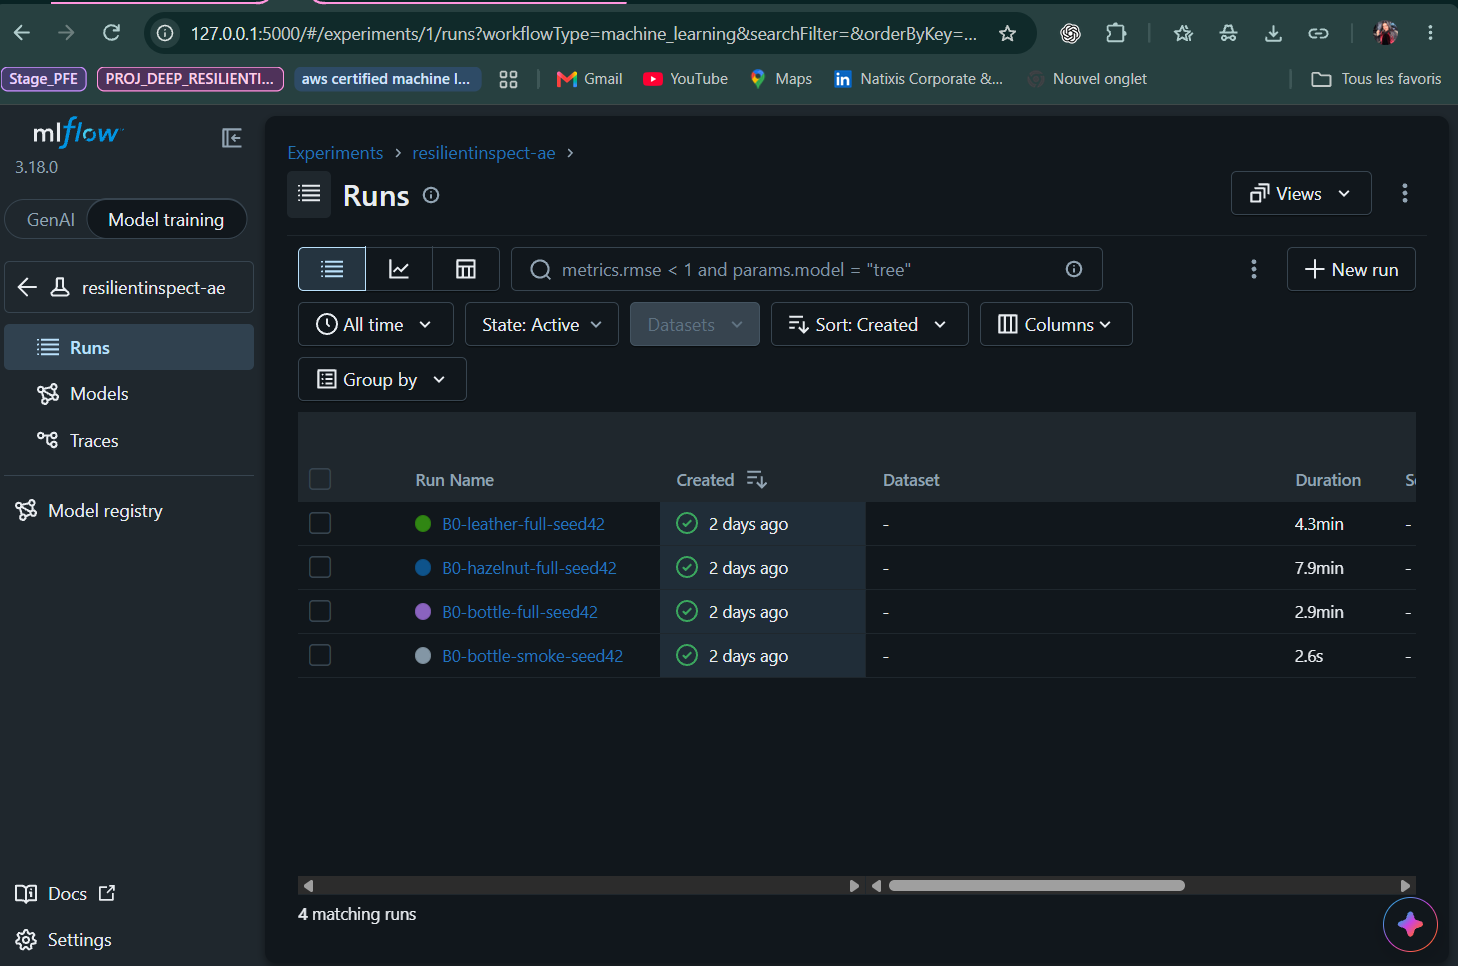
\includegraphics[width=\linewidth,trim=171bp 147bp 18bp 240bp,clip]{figures/mlflow_b0_capture.png}
\end{center}
\proofcaption{Capture réelle recadrée : trois runs B0 complets et un smoke, pas six. Les trois A1 complets sont confirmés par leur base MLflow et leurs artefacts, non par cette capture.}
\source{Source : \texttt{capture\_mlflow/6\_runs\_mlflow.png}. L'URL est une interface locale, non un service partagé.}

\vspace{3pt}
\textbf{B. Courbes d'apprentissage réelles B0 bottle}\par
\begin{minipage}[c]{0.70\linewidth}
\centering
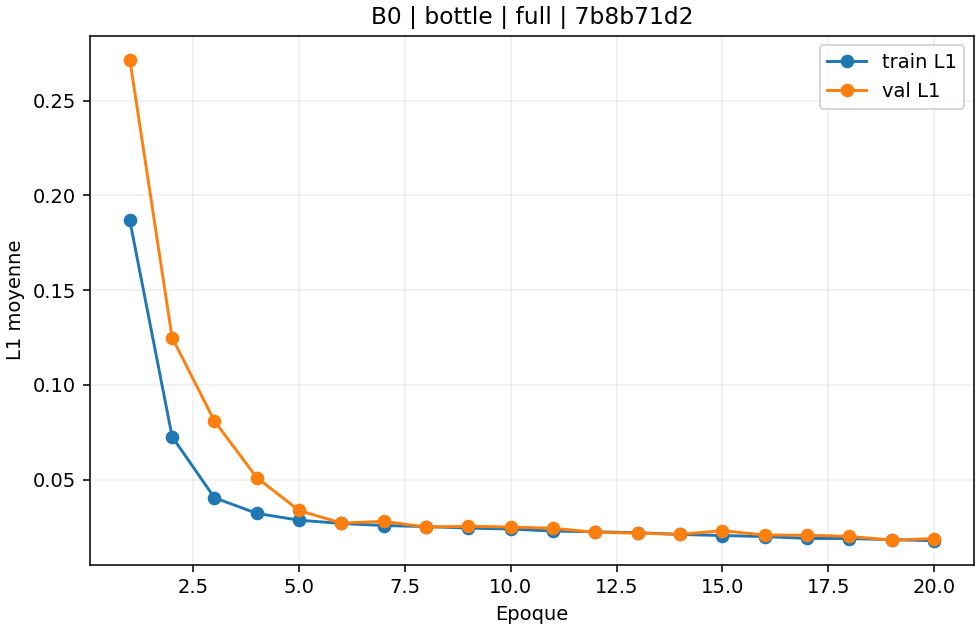
\includegraphics[width=\linewidth]{figures/b0_bottle_learning_curve.png}
\end{minipage}\hfill
\begin{minipage}[c]{0.27\linewidth}
\small
\textbf{Run :} \texttt{7b8b71d2}\par
20 époques réalisées.\par
Meilleur checkpoint : époque 19.\par
La sélection repose sur la perte val L1.\par
Ces courbes ne sont pas des métriques de détection.
\end{minipage}\par
\proofcaption{Courbes archivées du run complet, conformes à son \texttt{history.csv}. Elles documentent l'apprentissage, sans comparaison numérique avec la perte composite A1.}
\source{Source : \texttt{artifacts/b0\_runs/bottle/full\_7b8b71d28bc44868840ca50f4b16f4a1/loss\_curves.png}.}

\vspace{3pt}
\textbf{C. Résultat de localisation réel B0 hazelnut}
\par\begin{tabularx}{\linewidth}{@{}CCCC@{}}
\small Entrée RGB & \small Reconstruction & \small Erreur L1 RGB & \small Masque de référence\\
\end{tabularx}
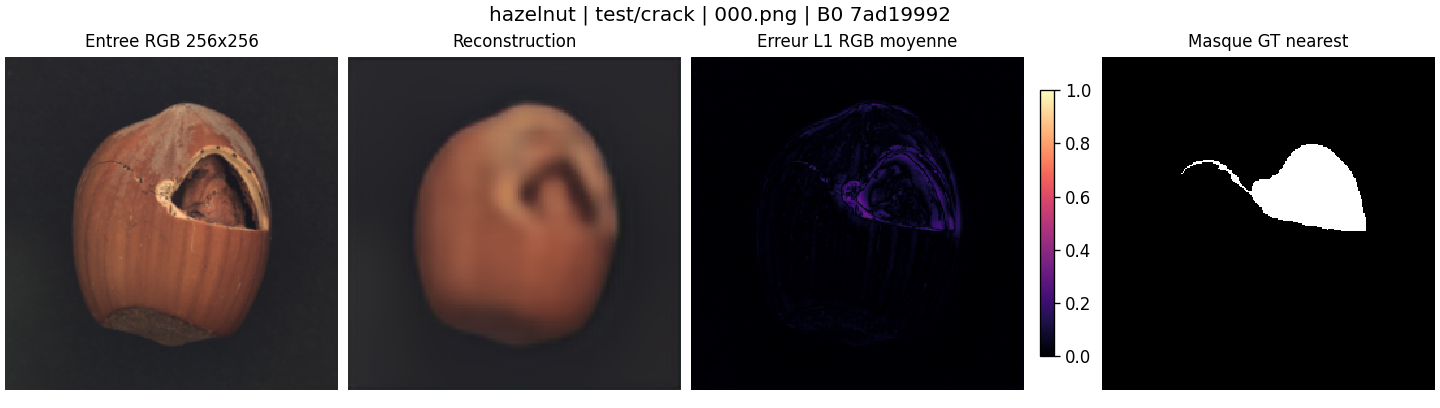
\includegraphics[width=\linewidth,trim=4bp 10bp 4bp 48bp,clip]{figures/b0_hazelnut_crack_000.png}
\proofcaption{Test \textit{hazelnut/crack/000.png}, run B0 \texttt{7ad19992}. Choix lexical fixé par le protocole, sans représentativité statistique revendiquée. La carte d'erreur n'est pas une carte Grad-CAM.}
\source{Source : \texttt{reports/evaluation/b0/f515662ab4ef/hazelnut/figures/crack\_000.png}. PNG source inchangé.}

\vspace{3pt}
\source{\textbf{Traçabilité.} Audit du 11/11/2026 ; commit \texttt{0d917a1} (09/11). Valeurs, sources et SHA joints sous \texttt{audit/}. Aucun entraînement ni test officiel relancé. MVTec AD : \url{https://www.mvtec.com/research-teaching/datasets/mvtec-ad}.}

\end{document}
